%\section{Beispielanhang}\label{Beispielanhang}
%Dieser Abschnitt dient nur dazu zu demonstrieren, wie ein Anhang aufgebaut seien kann.
%\subsection{Weitere Gliederungsebene}
%Auch eine zweite Gliederungsebene ist möglich.
%\section{Bilder}
%Auch mit Bildern.
%Diese tauchen nicht im Abbildungsverzeichnis auf.
%\begin{figure}[H]
%    \centering
%    \caption[]{Beispielbild}
%	\label{fig:Beispielbild}
%    \includegraphics[width=1\textwidth]{verzeichnisStruktur}
%\end{figure}

\section{Interviews}
\subsection{Interview: Use-Case-Identifikation}
\subsubsection{Interviewleitfaden}
\label{anhang:InterviewleitfadenUseCase}
\textbf{Identifikation eines geeigneten Use Cases für einen Copilot-Agenten in Dynamics 365 for Finance and Operations}

\vspace{0.5em}

\textbf{Einstieg}

Ich möchte gemeinsam mit dir herausfinden, welcher Use Case sich in \textit{Dynamics 365 for Finance and Operations (D365 FnO)} besonders gut für den Einsatz eines Copilot-Agenten eignet.

Das Gespräch dauert nur wenige Minuten und dient der Identifikation eines sinnvollen und relevanten Anwendungsszenarios.

\vspace{0.5em}

\textbf{Problem- und Prozessverständnis}

\begin{itemize}
    \item Welche Prozesse oder Aufgaben in D365 FnO empfindest du als besonders zeitintensiv, fehleranfällig oder umständlich?
\end{itemize}

\vspace{0.5em}

\textbf{Potenzial für Copilot-Unterstützung}

\begin{itemize}
    \item Wo siehst du grundsätzlich Potenzial für KI-Unterstützung durch einen Copilot-Agenten in D365 FnO?
    \item Welche Aufgaben könnten deiner Meinung nach gut automatisiert, vorbereitet oder durch Vorschläge unterstützt werden?
\end{itemize}

\vspace{0.5em}

\textbf{Identifikation eines konkreten Use Cases}

\begin{itemize}
    \item Wenn du einen einzigen Use Case auswählen müsstest, der am meisten Nutzen stiften würde, welcher wäre das?
    \item Warum ist gerade dieser Use Case aus deiner Sicht besonders geeignet für einen Copilot-Agenten?
\end{itemize}

\vspace{0.5em}

\textbf{Relevanz und Machbarkeit}

\begin{itemize}
    \item Gibt es aus deiner Sicht Gründe, die gegen die Umsetzung dieses Use Cases sprechen würden?
\end{itemize}

\vspace{0.5em}

\textbf{Abschluss}

\begin{itemize}
    \item Hast du sonst noch irgendwelche Anmerkungen?
\end{itemize}

\subsubsection{Interview 1}
\label{anhang:i1}
\textbf{Einleitung}\newline
Ich möchte gemeinsam mit dir herausfinden, welcher Use Case sich in D365 FnO besonders gut für den Einsatz eines Copilot-Agenten eignet.
Das Gespräch dauert nur wenige Minuten und dient der Identifikation eines sinnvollen und relevanten Anwendungsszenarios.

\textbf{Welche Prozesse oder Aufgaben in D365 FnO empfindest du als besonders zeitintensiv, fehleranfällig oder umständlich?}\newline
Für User ist die Anlage von großen Angeboten und Aufträgen zeitintensiv. Gerade die Artikelsuche ist hier immer ein Thema, da nicht immer alle wichtigen Daten zum Identifizieren des richtigen Artikels bekannt sind. Als Berater ist es umständlich Einrichtungen zu kopieren für welche keine technische Möglichkeit des kopieren bestehts also keine Entitäten vorhanden sind. Gerade in Projekten mit mehreren Mandanten ist dies sehr Zeitintensiv.

\textbf{Wo siehst du grundsätzlich Potenzial für KI-Unterstützung durch einen Copilot-Agenten in D365 FnO?}\newline
Für mich sehe ich viel Potenzial in der Unterstützung von neuen Usern. Eine Unterstützung bei der korrekten Anlage von Dokumenten wie Angeboten und Aufträgen sehe ich als potenziell hilfreich. Generell User, aber insbesondere auch neue User tendieren dazu Dokumente falsch anzulegen und dadurch den gesamten Vertriebsprozess am Beginn zu stören und dadurch Fehler und Mehrarbeit zu produzieren.

\textbf{Welche Aufgaben könnten deiner Meinung nach gut automatisiert, vorbereitet oder durch Vorschläge unterstützt werden?}\newline
Anlage von Dokumenten wie Auftrag, Angebot, Retoure.

\textbf{Wenn du einen einzigen Use Case auswählen müsstest, der am meisten Nutzen stiften würde, welcher wäre das?}\newline
Die Unterstützung der Angebotsanlage und damit verbunden die Artikelsuche.

\textbf{Warum ist gerade dieser Use Case aus deiner Sicht besonders geeignet für einen Copilot-Agenten?}\newline
Da er nicht zu komplex ist aber durch die große Nutzung der Angebotsfunktionen viel Mehrwert bieten kann.

\textbf{Gibt es aus deiner Sicht Gründe, die gegen die Umsetzung dieses Use Cases sprechen würden?}\newline
Ja die Fehleranfälligkeit kann zu einem Problem werden. Es ist wichtig, dass wenig Fehler
auftreten und wenn dies der Fall ist diese einfach zu identifizieren und nachzuvollziehen
sind. Ist dies nicht der Fall, schwindet die Userakzeptanz und der Agent wird nicht genutzt.

\textbf{Hast du sonst noch irgendwelche Anmerkungen?}\newline
Bei allen ERP Themen muss immer vom „unfähigsten“ User ausgegangen werden. Dies sind
im Projekt meist die User an denen solche Umsetzungen scheitern können.

\subsection{Interviews: Anforderungserhebung}
\subsubsection{Interviewleitfaden}
\label{anhang:InterviewleitfadenAnforderungserhebung}
\textbf{Anforderungen an einen Copilot-Agenten zur Unterstützung bei der Angebotsanlage in Dynamics 365 for Finance and Supply Chain Management}

\vspace{0.5em}

\textbf{Einstieg}

Für meine Bachelorarbeit entwickle ich einen Copilot-Agenten, der Anwender beim Anlegen eines neuen Angebots in D365 FnO unterstützen soll.

Der Agent soll dabei helfen, Angebotsfelder automatisch vorzubereiten, Werte vorzuschlagen oder Eingaben zu übernehmen.

Ziel des Interviews ist es, Herausforderungen und Anforderungen zu identifizieren, die für die Gestaltung des Agents relevant sind.

Das Gespräch dauert etwa 20 Minuten. Deine Aussagen werden anonymisiert ausgewertet.

\vspace{0.5em}

\textbf{Rollenverständnis}

\begin{itemize}
    \item Welche Rolle hast du im Kontext von D365 FnO, und wie vertraut bist du mit der Angebotserstellung?
\end{itemize}

\vspace{0.5em}

\textbf{Aktueller Ablauf und Herausforderungen}

\begin{itemize}
    \item Wie läuft das Anlegen eines neuen Angebots in D365 FnO aktuell typischerweise ab?
    \item Welche Schritte beim Ausfüllen der Angebotsfelder sind deiner Erfahrung nach besonders zeitaufwendig oder fehleranfällig?
    \item Welche Informationen werden beim Anlegen eines Angebots am häufigsten benötigt, und wo entstehen dabei typische Probleme?
\end{itemize}

\vspace{0.5em}

\textbf{Anforderungen an den Copilot-Agenten}

\begin{itemize}
    \item Was würdest du dir grundsätzlich von einem Copilot-Agenten wünschen, der beim Anlegen eines Angebots unterstützen soll?
    \item Auf welche Daten sollte der Agent zugreifen können, um sinnvolle Unterstützung zu bieten?
\end{itemize}

\vspace{0.5em}

\textbf{Gestaltung und Interaktion des Agents}

\begin{itemize}
    \item Wie sollte der Agent in D365 FnO verfügbar sein: als eigenes Fenster, als integriertes Panel im Formular oder in einer anderen Form?
    \item Wie stellst du dir die Interaktion mit dem Agenten vor?
    \item Wie wichtig ist es dir, dass der Agent seine Vorschläge begründet oder erklärt?
\end{itemize}

\vspace{0.5em}

\textbf{Risiken und offene Anforderungen}

\begin{itemize}
    \item Welche Risiken oder Herausforderungen siehst du beim Einsatz eines solchen Agents?
    \item Gibt es weitere Anforderungen oder Punkte, die für diesen Use Case berücksichtigt werden sollten?
\end{itemize}

\subsubsection{Interview 2}
\label{anhang:i2}
\textbf{Börgel, Damien}\newline
Genau, für meine Bachelorarbeit entwickle ich einen Copilot Agenten, der dem Anwender dann beim Anlegen von Angeboten in D365 Finance and Operations helfen soll.
Angebotsfelder automatisch vorzubereiten oder halt ne, je nachdem was jetzt die Anforderungen sind, das halt zu machen. Also vorbereiten, vorschlagen, auch ausfüllen und so, je nachdem, was das jetzt hier ergibt.

\textbf{Interviewter 2}\newline
Ja.

\textbf{Börgel, Damien}\newline
Ja, das ist dann das Ziel von dem Interview hier, dass wir ein bisschen was raussuchen und das soll so ungefähr 20 Minuten dauern. Plus minus konnte ich jetzt noch nicht so genau einschätzen und es wird natürlich alles anonymisiert.
Gut, fangen wir erst mit der ersten Frage an: Welche Rolle hast du mit Kontext mit D. 365 FNO und wie vertraut bist du mit der Angebotserstellung?

\textbf{Interviewter 2}\newline
Ja, welche Rolle? Also ich bin ja.
Im Bereich Vertrieb als Berater tätig, dass jetzt ja nun auch schon seit knapp 8 Jahren.
Und demnach ist der Angebotsprozess in den jeweiligen Projekten immer ein fester Bestandteil der Konzeptionierung oder der Ausarbeitung der Vertriebskonzepte, weshalb ich mich sehr gut damit auskenne. Der Angebotsprozess wird zwar auch immer gelebt, aber ist natürlich nicht so intensiv bei allen Kunden präsent, wie sag ich mal, der reine Verkaufsprozess. Aber er wird immerhin genutzt und Teilfunktionalitäten, die oder Funktionalitäten, die im Verkaufsauftrag
benötigt werden müssen, dann ja teilweise auch schon im Angebotsprozess greifen, weil falls ein Angebot dann gewandelt wird in einem Verkaufsauftrag, werden diese Funktionalitäten dort auch benötigt. Also müssen die teilweise ja
An die Stelle weitervererbt werden.

\textbf{Börgel, Damien}\newline
Super.
Ja, dann wäre direkt die erste Frage zum Thema des Angebots wieder aktuell, also mit mit D. 365 FNO selber, wie das so typischerweise abläuft, wenn man ein Angebot da drin erstellt.

\textbf{Interviewter 2}\newline
Identisch ist wie bei der Auftragserfassung oder Rücklieferungsauftragserfassung, dass entsprechend die Kundendaten oder der entsprechende Debitor gefunden wird.
das ist dann immer ja, je nachdem wie der Suchindex ist oder welche, welche Fragmente man zur Verfügung hat, wenn man nicht gerade die Kundennummer auswendig weiß, dass man da nach einem Namen suchen kann. Dann natürlich das direkte Anlegen per aktivem Klick auf "New". So, das ist natürlich immer etwas, was ausgefüllt werden muss. Dann hast du ja auch noch genau die die Auswahl, die da dir zur Verfügung steht. Ja, gut, ja, wenn wir dann den bestehenden Kunden nehmen, ja, besteht da dann die Herausforderung anhand von Adressdaten, Straße oder sonstiges, den Debitor herauszufinden, falls er mal keinen identischen Namen hat.
wie mehrere Kunden oder Niederlassung von Kunden, dass man den entsprechenden richtigen Datensatz auch auswählt.
Genau, dann die Auswahl der Auftragskategorie. Also, die kann man ja auch vorbelegen lassen, dass man sagt, wir haben ein Angebot und wir haben entsprechend eine Angebotskategorie, die wird vorbelegt. Die kann man dann entsprechend manuell auch abändern.
Das wird sich aber dann eigentlich auch aus dem Anlageprozess ergeben. Normalerweise hat man ja genau dafür schon vordefinierte Kategorien, dass man sagt, bei der manuellen Anlage nehmen wir das, wenn etwas von außen angelegt wird, automatisiert also über ein Journal, ne wie die Kategorie, also findet da erfahrungsgemäß relativ wenig ja Bewegung statt.
Alles andere ist durch die Konfiguration wie Standort, Lagerort auch vorbelegt, die Lieferdatumskontrolle ist natürlich auch ein Feld, das passend mit dem gewünschten Lieferdatum gefüllt werden muss. 
Ja, andere Informationen rein, Lieferart kann vielleicht in dem Angebot schon manuell ausgewählt werden, wenn feststeht, du, ich möchte 'n Angebot haben für Expresslieferung, für Spedition oder sonstiges, dann muss das natürlich anders gefüllt werden, als es standardmäßig gemacht wird.
Ja und wenn die Standardeinstellungen entsprechend vollzogen sind, klickst du den Button "OK".
Weitere Daten gibst du dann entsprechend Manuell einmal durch, weiß ich nicht, mit dem Kunden telefonierst.
kannst den Artikel eingeben und sagst, er möchte den und den oder du hast vorab 'ne E-Mail gekriegt und packst die Artikel per Drag and Drop rein aus der aus der E-Mail oder hast 'ne Excel-Vorlage, um die dort einzuspielen.
das wären so Dinge, die man dort berücksichtigen muss oder kann, um vielleicht Dinge auch zu automatisieren. Da natürlich drauf achten auf Artikelnummer und Stückzahlen, da die, wenn man die Artikelnummer nicht zur Hand hat, im System sehr, ja, anspruchsvoll sein kann.

\textbf{Börgel, Damien}\newline
Ok, also sind es im Prinzip viele einzelne Felder, die man einfach von A nach B übernehmen muss?

Sprecher1   11:17
Ja, genau.

\textbf{Börgel, Damien}\newline
OK. 
Ja da bist du schon ein wenig drauf eingangen, aber vielleicht nochmal, welche Schritte da noch erfahrungsgemäß besonders zeitaufwendig sind oder fehleranfällig ist da was bei?

\textbf{Interviewter 2}\newline
Ja, Artikelnummer ist immer so ein kritisches Ding, wenn dort ja.
Weil jemand selbst zu schnell ist oder nicht geduldig ist oder die Suche vorab aufgeht, bevor man schon angefangen hat zu tippen. Oder während des Tippens geht dann der Suchindex schon auf und schlägt dann die ganze Batterie von Artikeln vor. Wäre natürlich cooler, wenn man das entsprechend schon direkt vorbelegt oder vorbelegen kann, durch entsprechende Inhalte, die bekannt sind.
Ähm.
Ja, individuell kommen natürlich noch hier Debitorenbestellungen oder ein Kommentartext noch rein in die Kopfzeile vom Kunden, dass man sieht, O. K., gibt es da vielleicht schon 'ne Bestellnummer zu oder 'ne Referenznummer?
Worauf der Kunde sich beziehen wird, was dann ja auch wieder automatisiert oder generell an die an den Verkaufsauftrag mit übernommen wird, wenn der denn dann zustande kommt.
Vielleicht noch 'ne abweichende Lieferadresse.
könnte noch so 'n Thema sein, je nachdem welche Filiale, für welche Filiale du gerade das Angebot erfasst, weil kann ja auch sein, dass 'n Debitor mehrere Lieferadressen hat, dann musst du natürlich wissen, für welche Lieferadresse, also wenn du das manuell anlegst, weil von außen ist vielleicht 'n bisschen einfacher, weil wir dann 'ne Standortkennung haben oder zumindest schon Trigger, welche Lieferadresse ist gemeint. Wenn du es aber manuell auswählst, sieht er die Standardlieferadresse vorbelegt, so und da das muss im Telefonat ja auch erfragen.
Ist die Lieferadresse korrekt, die da vorbelegt ist, oder möchtest du die Lieferung zu einem zu einem zu einer anderen Lieferadresse haben? Das wäre vielleicht noch mal so eine Frage, die da aufploppen könnte, sollte.

\textbf{Börgel, Damien}\newline
Ja, Ok.
Gut, dann die nächste Frage. Die hattest die hast du, glaub ich, dann nämlich schon bei der ersten Frage beantwortet, weil das dann welche Informationen am häufigsten benötigt werden. Das hast du ja grade eigentlich alles schon aufgezählt.

\textbf{Interviewter 2}\newline
Ja.

\textbf{Börgel, Damien}\newline
Genau, und dann kommen wir nämlich eigentlich zur, ja, ich sag mal, wichtigsten Frage. Wie genau man so einen Agenten einbauen könnte, der da unterstützt. Ich glaub, du hast gerade schon viele Sachen gesagt, die vielleicht halt nicht so gut oder ne, wo es Probleme geben könnte und wie und wo genau da vielleicht so ein Agent unterstützen könnte. Beispiele wären jetzt zum Beispiel, dass das halt

\textbf{Interviewter 2}\newline
Mhm.
Ja, also es wäre gut, wenn der Agent direkt für einen die Angebote anlegt, ja, also, dass direkt auch die wichtigsten Felder mit ausfüllt und damit dann auch bei der Suche von Artikeln hilft.
Das
Ja, ich wüsste jetzt nicht, was noch für Varianten gibt, ah, vielleicht doch eine eine Sache fällt mir noch auf, wenn wir manuelle Angebote eingeben und wir haben Artikelersetzung oder Mengen Vorgaben, die pro Artikelnummer und dann geht ja immer so 'n Abfragekontext auf der bestätigt werden muss, ob wir das übernehmen möchten oder nicht. Das kann auch noch mal 'ne Aufgabe sein, die dann so 'n Agent übernehmen muss oder ja, die Berechtigung dazu haben muss, diese Bestätigung auszufüllen, wenn ich das denn möchte.

\textbf{Börgel, Damien}\newline
Yep, OK.

\textbf{Interviewter 2}\newline
Weil da müssen wir auch aktiv reinklicken und sagen, ja, akzeptieren wir oder ignorieren wir. Und das muss der Agent dann auch können.

\textbf{Börgel, Damien}\newline
Yeah, OK.
Gut.
Ja, also wären quasi die 3 Dinger, dass der Agent dasselbe anlegt, dass der Agent suche, wenn beim Suchen quasi hilft, Artikel oder Kundennummer oder was auch immer.

\textbf{Interviewter 2}\newline
Ja.

\textbf{Börgel, Damien}\newline
OK.

\textbf{Interviewter 2}\newline
Und.

\textbf{Börgel, Damien}\newline
Und halt ja, das ja.

\textbf{Interviewter 2}\newline
Was ebenfalls noch.
Noch wünschenswert ist, wenn dann so ein Angebot vor Ablauf ist.
Weiß nicht, ob es das ja.
Ob das dann wieder Herr ist, wahrscheinlich dann ein anderer Agent, der einen daran erinnert, entsprechend.

\textbf{Börgel, Damien}\newline
Ja, das wär ein anderer.

\textbf{Interviewter 2}\newline
Das wäre ein anderer Agent, ja.

\textbf{Börgel, Damien}\newline
So.

\textbf{Interviewter 2}\newline
Ist wahrscheinlich auch wiederum ein anderer Agent, der das Angebot wandelt.

\textbf{Börgel, Damien}\newline
Yeah.
Das wären alles so Dinge, die man hintereinander quasi schalten würde, was wir aber gerade noch.

Sprecher1   17:19
Ja, wandeln, stornieren, genau.

\textbf{Börgel, Damien}\newline
Komm, dass du hast ja gesagt, also ein paar Sachen irgendwie, wenn die Lieferadresse abweicht und sowas.

\textbf{Interviewter 2}\newline
Mhm.

\textbf{Börgel, Damien}\newline
Dass sowas alles passieren kann, man könnte ja theoretisch bei dem Agenten auch mit einbauen, dass der quasi, dass der während man mit dem Kunden telefoniert, dass man den quasi als Chatbot auch benutzen kann. wo er dann vielleicht Unterstützung liefert oder

\textbf{Interviewter 2}\newline
Ja.

\textbf{Börgel, Damien}\newline
Hatte ich vorher noch gar nicht so im Sinn.

\textbf{Interviewter 2}\newline
Das wäre.
Das wäre auch mit Sicherheit.
Eine gute Aktion, aber.
Jetzt überlege ich gerade.
Ja, doch, auf jeden Fall, mein ganz normale Prozess.
Weil das Telefon klingelt ja zum Glück beim Kunden auch noch zwischendurch.
Ist auch relativ wenig, aber dieses beim Telefonprozess oder bei telefonischen Bestellungen den da durchzuleiten.
Ist sicherlich auch interessant. Hast du den Vertrieb direkt nicht mehr am Telefon?
und der Vertrieb greift dann nur aktiv ein, falls ja, der Agent irgendwie mit den Eingabeaufforderungen nicht weiterkommt oder der Kunde aktiv sagt, boah nee, das Ergebnis da von dem Angebot gefällt mir gar nicht, ich möchte.
Möchte bitte mit einer realen Person verbunden werden.

\textbf{Börgel, Damien}\newline
No.
Ja gut, oder dass die reale Person das quasi dann im Hintergrund hat. Ne, geht ja auch, dass das dann quasi ne so unterstützend, dass dann quasi währenddessen die Sachen da eingetragen werden können und dann wird immer zwischendurch nachgefragt: 'Hier, möchtest du da noch was haben? Möchtest du da noch was haben, damit nichts vergessen wird?'

\textbf{Interviewter 2}\newline
Ja ja, genau so meine ich das. Obwohl das wahrscheinlich nur eine Anfangslösung wäre, weil langfristig ist das ja eigentlich unnötig, weil dafür ist der Agent ja da, dass da nicht nur jemand beisitzt und die ganze Zeit prüft, macht er das richtig. Das kannst du vielleicht machen für Trainingszwecken, dass er, dass er das überprüft, ob das alles richtig ist. Aber normalerweise sollte dann ja der reine Vertriebsmitarbeiter eigentlich gar nicht mehr eingreifen, sondern nur irgendwie per Chatnachricht per Chatbot benachrichtigt werden. Achtung, hier Vertrieb XY Customer Service.
Kunde aus Webshop benötigt trotz Assistenten Fachkraftunterstützung. 

\textbf{Börgel, Damien}\newline
OK. 
Ja, dann direkt die nächsten Fragen, wie genau der Agent verfügbar sein soll, also ob der.
Oder würd ich, glaub ich, Frage 8 einmal vorziehen. Wie genau der Agent, also wie genau die Interaktion mit dem Agenten Funktionieren soll, weil ich glaube, da gehst du ja schon in 'ne ziemlich spezifische Richtung, dass das nicht mehr dann was ist, wo dann der Vertriebsmitarbeiter selber mitarbeitet, sondern dass der quasi automatisiert arbeitet.
Sprich.
Ja, einfach direkt die Verarbeitung von externen Eingaben, dass das dann im Prinzip das Ziel ist, richtig?

\textbf{Interviewter 2}\newline
Ja, genau. Also würde ich sagen, dass etwas gebraucht, womit ein Kunde ein Angebot anlegen kann, ohne Probleme. Dass Unterstützung dich einen Agenten gegeben wird, dabei. Das kann dann ja auch für Lernzwecke für Vertriebler genutzt werden.
Ja, und sonst weiß ich nicht, einen Agenten. Was kannst du sonst noch für einen Agenten nehmen?
Ja, da geht es ja wirklich jetzt rein darum, dass der die Eingaben.
erledigt oder 'ne Eingabenaufforderung erledigt, die vom Kunden vorgegeben wird. So, ich weiß nicht, ob der gleiche Agent auch die Sachen prüft und erledigt, wenn eins von außen angelegt wird, weil dann ist das Angebot ja schon angelegt.
Dann kann er maximal noch prüfen, ob die Eingaben richtig sind.
Wer die dann korrigiert, aber das haben wir ja eigentlich schon mit unserer Prozessstatusfolge oder mit den Prüfbedingungen abgeschlossen, ne?

\textbf{Börgel, Damien}\newline
Ja, das kommt dann alles danach.

\textbf{Interviewter 2}\newline
Dass dann der Prozess, warum der Prozess nicht durchgeht, und dann ist für mich wieder kommt wieder ein anderer Agent oder sonstiges.
zum Tragen, der dann zum Beispiel sagt, das Angebot ist irgendwie nicht, ist nicht in dem finalen Prozessstatus, anstatt diese Kachel, die wir dann haben, dann hast du den Agenten, der die Kacheln überwacht und dir vielleicht 'ne Nachricht schickt.
Und dich aktiv darauf aufmerksam macht: "Ey, ruf mal Kunde XY an. Hier die Wandlung von außen hat nicht funktioniert. Da sind irgendwelche Eingaben falsch."

\textbf{Börgel, Damien}\newline
Hm.

\textbf{Interviewter 2}\newline
Dann eher so n so n so n Workflow, der dann stattfinden muss, ne als dass du dafür n Agenten vielleicht brauchst.

\textbf{Börgel, Damien}\newline
Ja.

\textbf{Interviewter 2}\newline
Also, einen Agenten kannst du ja wirklich dann nutzen, wenn der.
Wirklich aktiv Eingaben.
erledigt, die du ihm mitgibst oder der dann vielleicht E-Mails verarbeitet. Also, ich kann mir diesen Einsatz von diesem Agenten bei E-Mail-Verkehr oder beim Chat vorstellen. Wenn ein Kunde also nicht auch chattet oder wie auch immer, was für Anbindungen die Kunden haben, dass er daraus die Informationen ableitet und dann ein Angebot erstellt. Ja, oder wie gesagt, aus einer konkreten E-Mail.

\textbf{Börgel, Damien}\newline
Ja. Ok.

\textbf{Interviewter 2}\newline
Nur dann muss ja auch vorhanden, da muss der Agent auch prüfen, ist sind die Inhalte in der E-Mail auch ja so wandelbar oder so vollständig, dass er überhaupt in der Lage ist bis zum Endprozess zu kommen, weil wenn er da nicht weiterkommt.

\textbf{Börgel, Damien}\newline
Ok.

\textbf{Interviewter 2}\newline
Was ist dann das Nächste? Schickt er dann dem?
Vertriebsindienste Nachricht, Achtung, ausgelesene E-Mail ist nicht vollständig, kann kann ich bearbeiten oder soll er dann 'ne E-Mail an den Kunden schreiben, lieber Kunde, deine E-Mail enthält keine schlüssigen Daten, was genau wolltest du haben?

\textbf{Börgel, Damien}\newline
Mhm.

\textbf{Interviewter 2}\newline
Deswegen ist immer, glaube ich, je Kanal auch dann wiederum andere.
Andere, sag ich mal, Funktionen oder andere Handlungsstränge sind notwendig.
Und wieder auch andere Berechtigung.

\textbf{Börgel, Damien}\newline
Ja, ich glaub damit, was du gerade sagst, gehst du auch direkt schon auf die nächste Frage dann drauf ein, was halt die Risiken und Herausforderungen von so einem Agenten wären und das ist ja genau das, was du gerade gesagt hast, ne? Was macht der bei falschen Werten?

\textbf{Interviewter 2}\newline
ja genau, der also der muss ja erstmal nach, genau, der muss ja nach, je nach Kanal muss er ja auch agieren können. So und das eine ist, ich habe jemanden live in der Leitung, der ad hoc antwortet, das andere ist, ich habe keinen Vis-a-vis-Austausch, sondern reagiere auf einen Datensatz, der da liegt.
Heißt, ich habe keinen Austauschpartner, sondern das mache ich dann mit einer genau, wie ich gerade sagte, vorliegenden E-Mail. In welcher Form auch immer.
oder was soll er dann tun? Soll er auch auf diese E-Mail antworten? Das heißt, braucht Berechtigungen auf Outlook, braucht die Berechtigung, eine E-Mail zu verfassen und zu schreiben und zu schicken.

\textbf{Börgel, Damien}\newline
Ja.
Mhm.
Ja, dann wäre die letzte Frage, ob du noch irgendwelche anderen hast.
Anmerkungen, Anforderungen, Punkte hast.

\textbf{Interviewter 2}\newline
Jetzt unabhängig vom Angebot oder wie?

\textbf{Börgel, Damien}\newline
Nö, zu dem Use Case jetzt selber, also zu den Angeboten.
Du kannst auch ja kurze Runde, bin ich was dazu sagen. Generell vielleicht zum Thema kann ich vielleicht auch benutzen.

\textbf{Interviewter 2}\newline
Mhm.
Doch, den kannst du ja, wenn ich jetzt überlege, es ruft ein Kunde an.
Also je nachdem, wie es vorgelagert ist, aber. Angenommen, es ruft jetzt ein Kunde an, der noch kein Kunde ist, der ein Angebot haben will, dann muss ja auch vorab schon die.
Die Frage kommen: Bist du ein Neukunde oder bist du ein Bestandskunde?
So, und wenn er dann Bestandskunde ist, kann er ja Daten nehmen und die abgleichen, wenn er kein Bestandskunde ist. Und wir lassen das Erfassen von einmal Kundendaten zu. Der muss ja die Felder ja auch alle entsprechend befüllen.
automatisiert.
Da muss ja die Daten alle abfragen, die.
Die man für so eine einmal Kundenerfassung dann bräuchte.

\textbf{Börgel, Damien}\newline
Mhm.

\textbf{Interviewter 2}\newline
Und dann muss ja ein weiterer Workflow ausgelöst werden. Sollte es ein Angebot geben für einen Interessenten, der bis dato nicht bekannt ist.
Muss dieser Agent ja auch. Entweder in diesem Prozess schon sofort.
Ein Vertriebsmitarbeiter. Hinzu ziehen und vielleicht.
Die Betreuung schon von da ab perfekt zu machen.
Und den Neukunden tatsächlich zu gewinnen. Oder reicht es für eine blanke Vorerfassung und der Agent sagt: Ja, vielen Dank für Ihr Interesse an unseren Produkten. Wir nehmen Ihre Daten auf und ein Vertriebs.
Ein Mitarbeiter aus dem Innendienst wird sich nach Sichtung Ihrer Kontaktaufnahme direkt melden. Ich glaube, da gibt es unterschiedliche Cases, die man abbilden kann, je nachdem, was das Unternehmen wünscht und inwiefern es auch umsetzbar ist, ne?

\textbf{Börgel, Damien}\newline
Ja.

\textbf{Interviewter 2}\newline
Da müsste man vielleicht auch gucken, welche Fragen man damit etabliert.
Weil, wenn ein Kunde.
Oder Interessent vielleicht vorliegt, hat ein Interessent.
Ja, weiß ich nicht. Hat er immer die Artikelnummern? Hat er die nicht? Also, ich glaube. Da kannst du davon bis spinnen, ne?

\textbf{Börgel, Damien}\newline
Jo.
Da kannst du, es geht noch tief rein.

\textbf{Interviewter 2}\newline
Ja.
Aber jetzt gehen wir mal von dem Best Case aus, der wer kennt die Artikelnummern und kennt auch alles Identische, aber auch dann muss er ja die ganzen Datensätze, die für Interessenten auszufüllen sind, abarbeiten.
Und dann weiter fortfahren. 
So, gibt es eine Preisliste für Interessenten oder macht man dann gar kein Angebot final fertig, sondern macht nur die Hülle, so dass dann der Indienst das sichtet und dann den Neukunden kontaktiert?
und dann im Nachgang hingeht, sagt: 'Hier, lieber Kunde, du hast über unseren Agenten ein Angebot angefordert, über die und die Artikel.'
Wir haben die und die Kundendaten, die wollten wir gerne abgleichen.
Weiß ich nicht, Umsatzpotenziale, Regionen, was nicht alles da noch hinzukommen kann.

\textbf{Börgel, Damien}\newline
Ja wenn du sonst nicht hast, dann sind wir durch.

\textbf{Interviewter 2}\newline
Ja, gucke mal.

\textbf{Börgel, Damien}\newline
Dann bedanke ich mich.

\textbf{Interviewter 2}\newline
Ja, gerne. Also, ich würde mich vielleicht tatsächlich mal dran, mit dem einfachsten Fall dann beschäftigen, für Agenten, einfach davon ausgehen, dass alles andere existiert.
Wie Preislisten und Artikelnummern sind bekannt, so dass man einfach mal den einfachsten Fall abbildet, um einmal einen Grundprozess auszuprobieren, ob das überhaupt Sinn macht oder nicht, das einzubauen.

\textbf{Börgel, Damien}\newline
Ok.

\textbf{Interviewter 2}\newline
Ah und was mir noch einfällt, es macht vielleicht noch Sinn Sachen abzuändern, also zum Beispiel andere Telefonnummer, worunter der erreichbar ist, als hier Zustellhinweis oder so, wenn das mal mit den Adressfeldern ein bisschen spielt oder auch mit den Referenzen. 
Dass man dann auch sagt, den Zustellhinweis, der Agent füllt füllt dann 'n Zustellhinweis aus, wie bitte bei der Nachbarin dienstags um 15:00 Uhr an der Hausnummer so und so abgeben.
Und dann vielleicht auch noch mal, falls die Eingabe da muss man ja auch immer drauf reagieren, falls die Eingabe von außen.
Falls ihr sagt "Oh Mist, meine letzte Eingabe war falsch", ist nicht Hausnummer 15, sondern 17.
Ja, weil alles, was wir sehen, wenn Menschen am Telefon sitzen, sagt man: "Ah nee, Mist, hab mich vertan. Ich brauch nicht ein, ich brauch zwei Stück." Oder: "Ach, Mist, ist auch nicht Eichendorffstraße, sondern Eisenbahnstraße."

\textbf{Börgel, Damien}\newline
Ja.
Also quasi im Endeffekt noch möglich ist, das Ding abzuändern, wenn irgendwas falsch eingefügt wird.

\textbf{Interviewter 2}\newline
Genau, dass der Agent, genau dass der Agent, genau dass der Agent darauf reagiert, wenn der Mensch sagt: 'Oh, meine letzte Angabe für die zuständigen Hinweise war falsch. Bitte korrigiere.'

\textbf{Börgel, Damien}\newline
Ok. Danke dir!

\subsubsection{Interview 3}
\label{anhang:i3}
\textbf{Einstieg}\newline
Für meine Bachelorarbeit entwickle ich einen Copilot-Agenten, der Anwender beim Anlegen eines neuen Angebots in D365 FnO unterstützen soll.
Der Agent soll dabei helfen, Angebotsfelder automatisch vorzubereiten, Werte vorzuschlagen oder Eingaben zu übernehmen.
Ziel des Interviews ist es, Herausforderungen und Anforderungen zu identifizieren, die für die Gestaltung des Agents relevant sind.
Das Gespräch dauert etwa 20 Minuten. Deine Aussagen werden anonymisiert ausgewertet.

\textbf{Welche Rolle hast du im Kontext von D365 FnO, und wie vertraut bist du mit der Angebotserstellung?}\newline
Ich bin Consultant für D365 für den Fachbereich Sales and Distribution und aktuell Teilprojektleiter Verkauf im Projekt Genesis (SABAG). Mit der Angebotserstellung bin ich sehr gut vertraut. 

\textbf{Wie läuft das Anlegen eines neuen Angebots in D365 FnO aktuell typischerweise ab?}\newline
 
\textbf{Welche Schritte beim Ausfüllen der Angebotsfelder sind deiner Erfahrung nach besonders zeitaufwendig oder fehleranfällig?}\newline
Das Erfassen von Feldern, welche nicht obligatorisch für das System sind, aber vom Kunden gewünscht sind wie Debitorenreferenzen oder Notizen an den Angebotspositionen.

\textbf{Welche Informationen werden beim Anlegen eines Angebots am häufigsten benötigt, und wo entstehen dabei typische Probleme?}\newline
Die wichtigsten Informationen im Angebot sind die Artikel und die Preise. Die typischen
Probleme entstehen bei der Artikelsuche. Diese ist architekturbedingt recht träge und
nimmt bei Fehlangaben viel Zeit in anspruch.
\textbf{Was würdest du dir grundsätzlich von einem Copilot-Agenten wünschen, der beim Anlegen eines Angebots unterstützen soll?}\newline
Meine Vorstellung wäre, dass der Agent Angebotsköpfe erstellen kann. Er sollte auf Basis
der Userinteraktion differenzieren können um welchen Angebotstyp es sich handelt. Bei
den Angebotspositionen sollte der Agent die Artikelsuche unterstützen und bestenfalls
Preishistorien aufzeigen können. Dadurch würde viel Aufwand erspart werden können. Bei der Preishistorie meine ich zu welchem Preis der Artikel in der Vergangenheit angeboten wurde oder zu welchem Preis andere Debitoren
diesen bezogen haben. 

\textbf{Auf welche Daten sollte der Agent zugreifen können, um sinnvolle Unterstützung zu bieten?}\newline
Auf Stammdaten aus D365 wie die Debitorenstammdaten, Artikelstammdaten inkl.
Wiederbeschaffungszeiten. Er sollte auf Lagerbestände zugriff haben und auf
Bewegungsdaten wie alle Angebote und ggf. alle Aufträge.

\textbf{Wie sollte der Agent in D365 FnSCM verfügbar sein: als eigenes Fenster, als integriertes Panel im Formular oder in einer anderen Form?}\newline
Der Agent sollte bestenfalls in D365 FnSCM als eigenes Fenster verfügbar sein. Somit kann der User direkt mit ihm interagieren, ohne in die entsprechenden Formulare abzuspringen.

\textbf{Wie stellst du dir die Interaktion mit dem Agenten vor?}\newline
Chat Interface und als Ausbaustufe die Verarbeitung  externer Eingaben

\textbf{Wie wichtig ist es dir, dass der Agent seine Vorschläge begründet oder erklärt?}\newline
M.M.n. zwingend notwendig um die Akzeptanz der User zu gewährleisten

\textbf{Welche Risiken oder Herausforderungen siehst du beim Einsatz eines solchen Agents?}\newline
Die größte Herausforderung ist, dass der Agent bei der Anlage von Angeboten, keine Fehler groben Fehler machen darf. Ein User wird den Agenten nie wieder nutzen, wenn er sich nicht sicher sein kann, dass der Output gut ist. Wenn Fehler auftreten, müssen diese zumindest leicht erkennbar und nachvollziehbar sein.

\textbf{Gibt es weitere Anforderungen oder Punkte, die für diesen Use Case berücksichtigt werden sollten?}\newline
Ich denke zu beginn sollte die Funktion nicht allzu umfangreich sein, sondern die
vorhandenen Funktionen optimal funktionieren. Es sollte die Qualität und nicht die
Quantität im Vordergrund stehen.

\section{Copilot Studio Screenshots}

\begin{figure}[H]
    \centering
    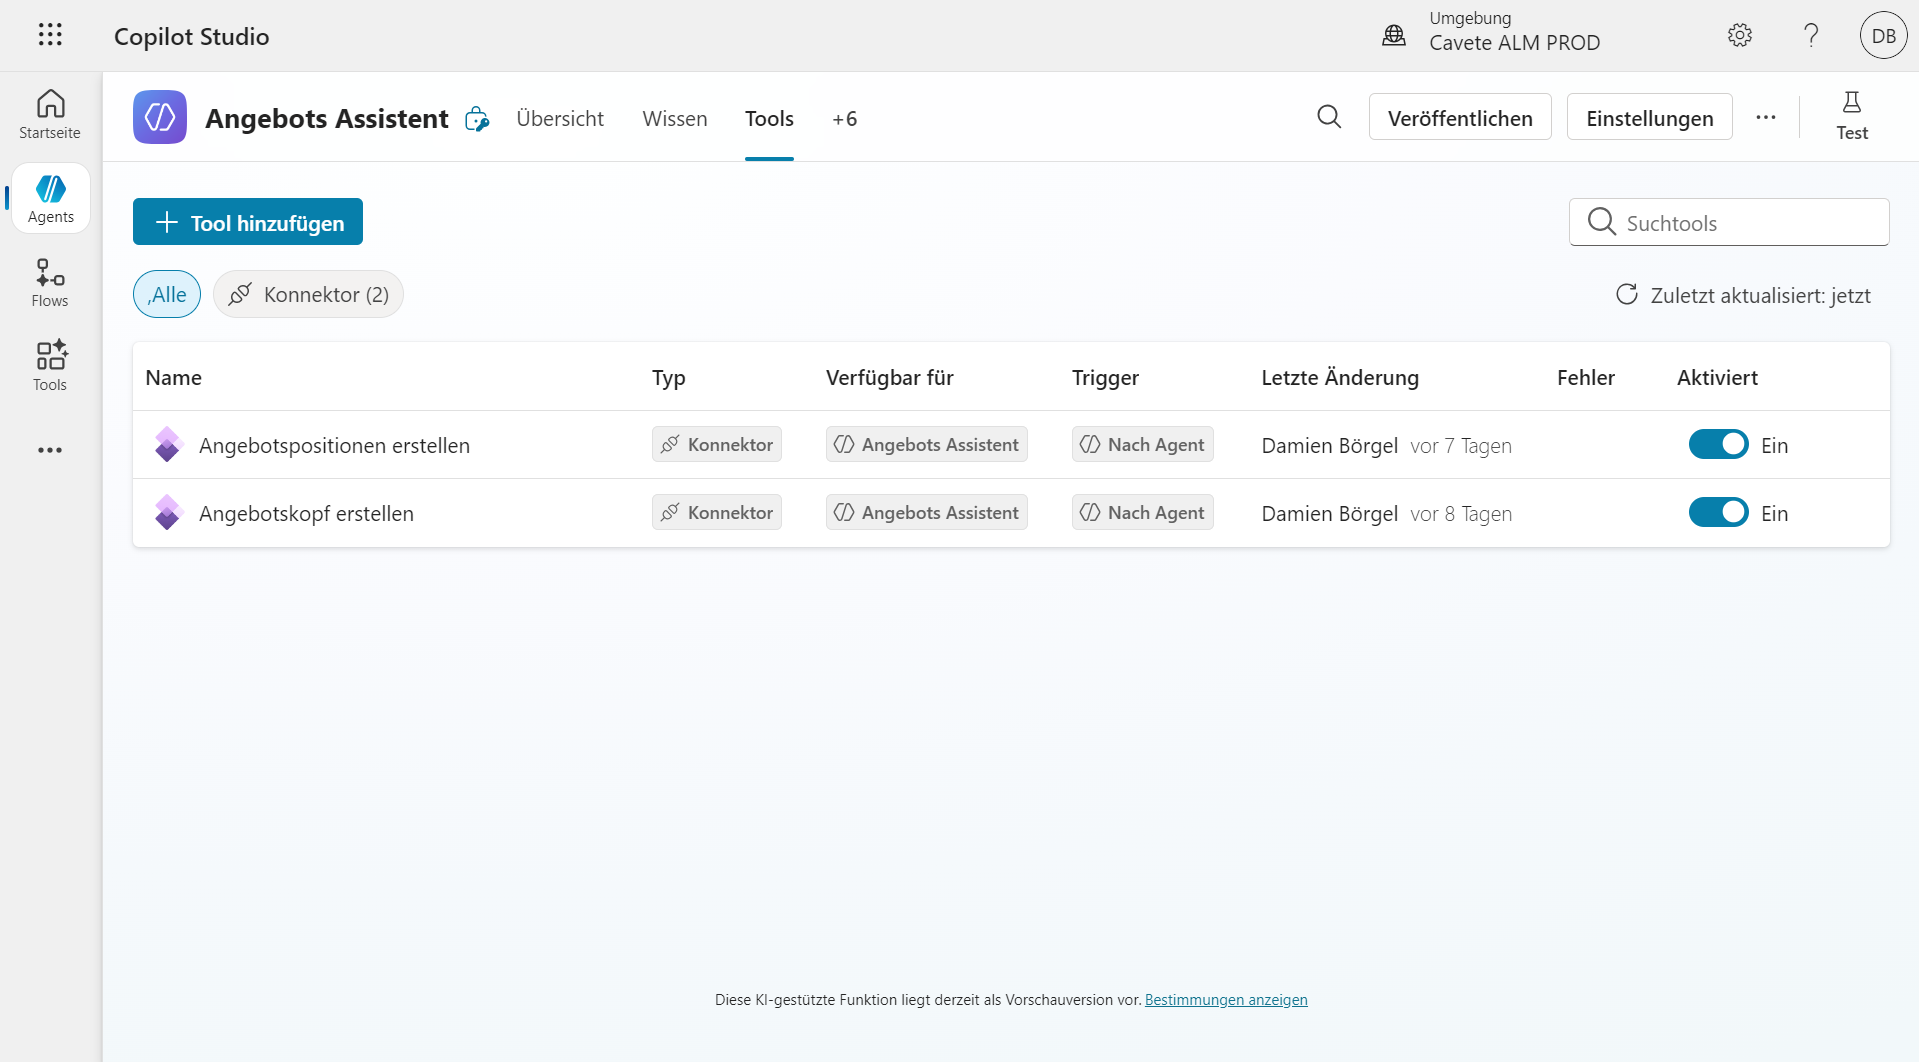
\includegraphics[width=1\textwidth]{kapitel/anhang/images/Tools.png}
    \caption{Übersicht der Tools}
    \label{fig:Tools}
\end{figure}

\begin{figure}[H]
    \centering
    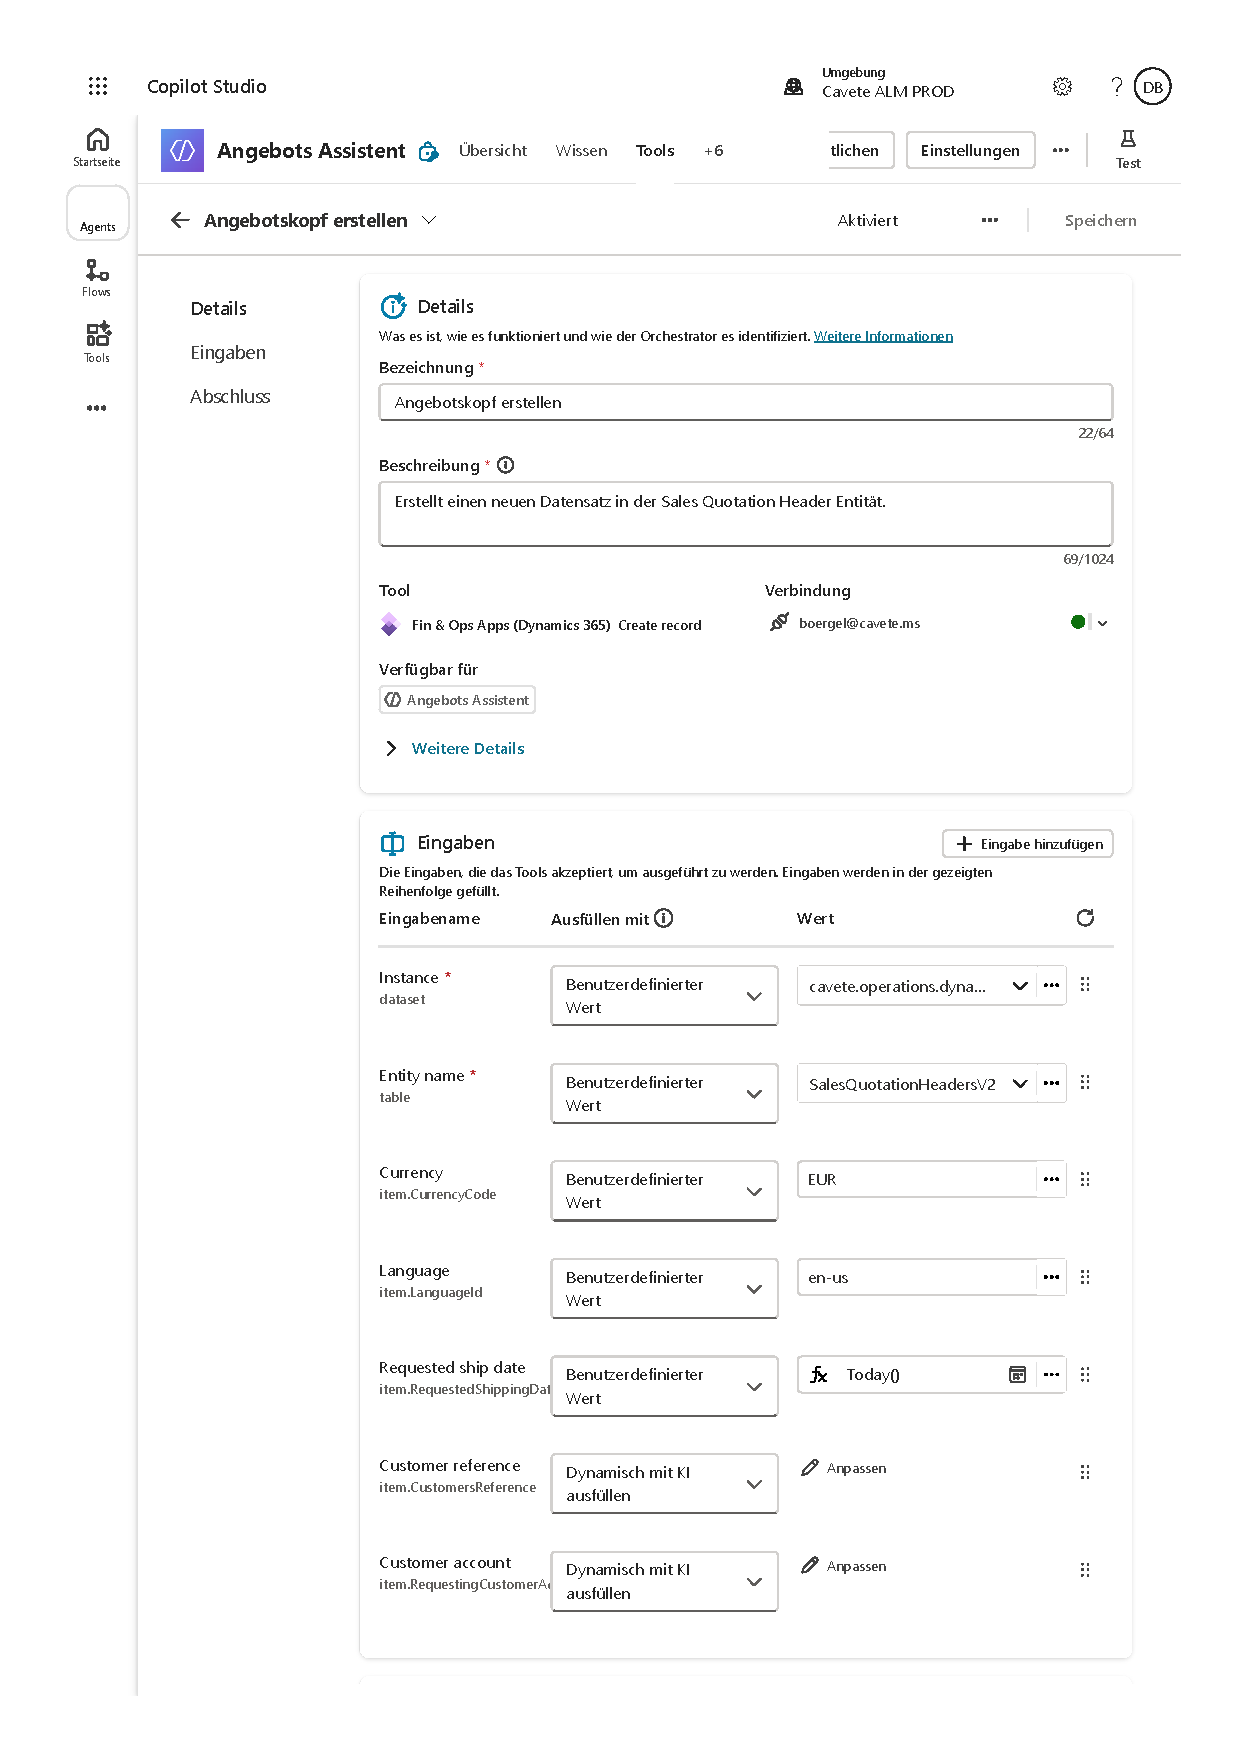
\includegraphics[width=1\textwidth]{kapitel/anhang/images/Angebotskopf.pdf}
    \caption{Tool: Angebotskopf erstellen}
    \label{fig:Angebotskopf}
\end{figure}   

\begin{figure}[H]
    \centering
    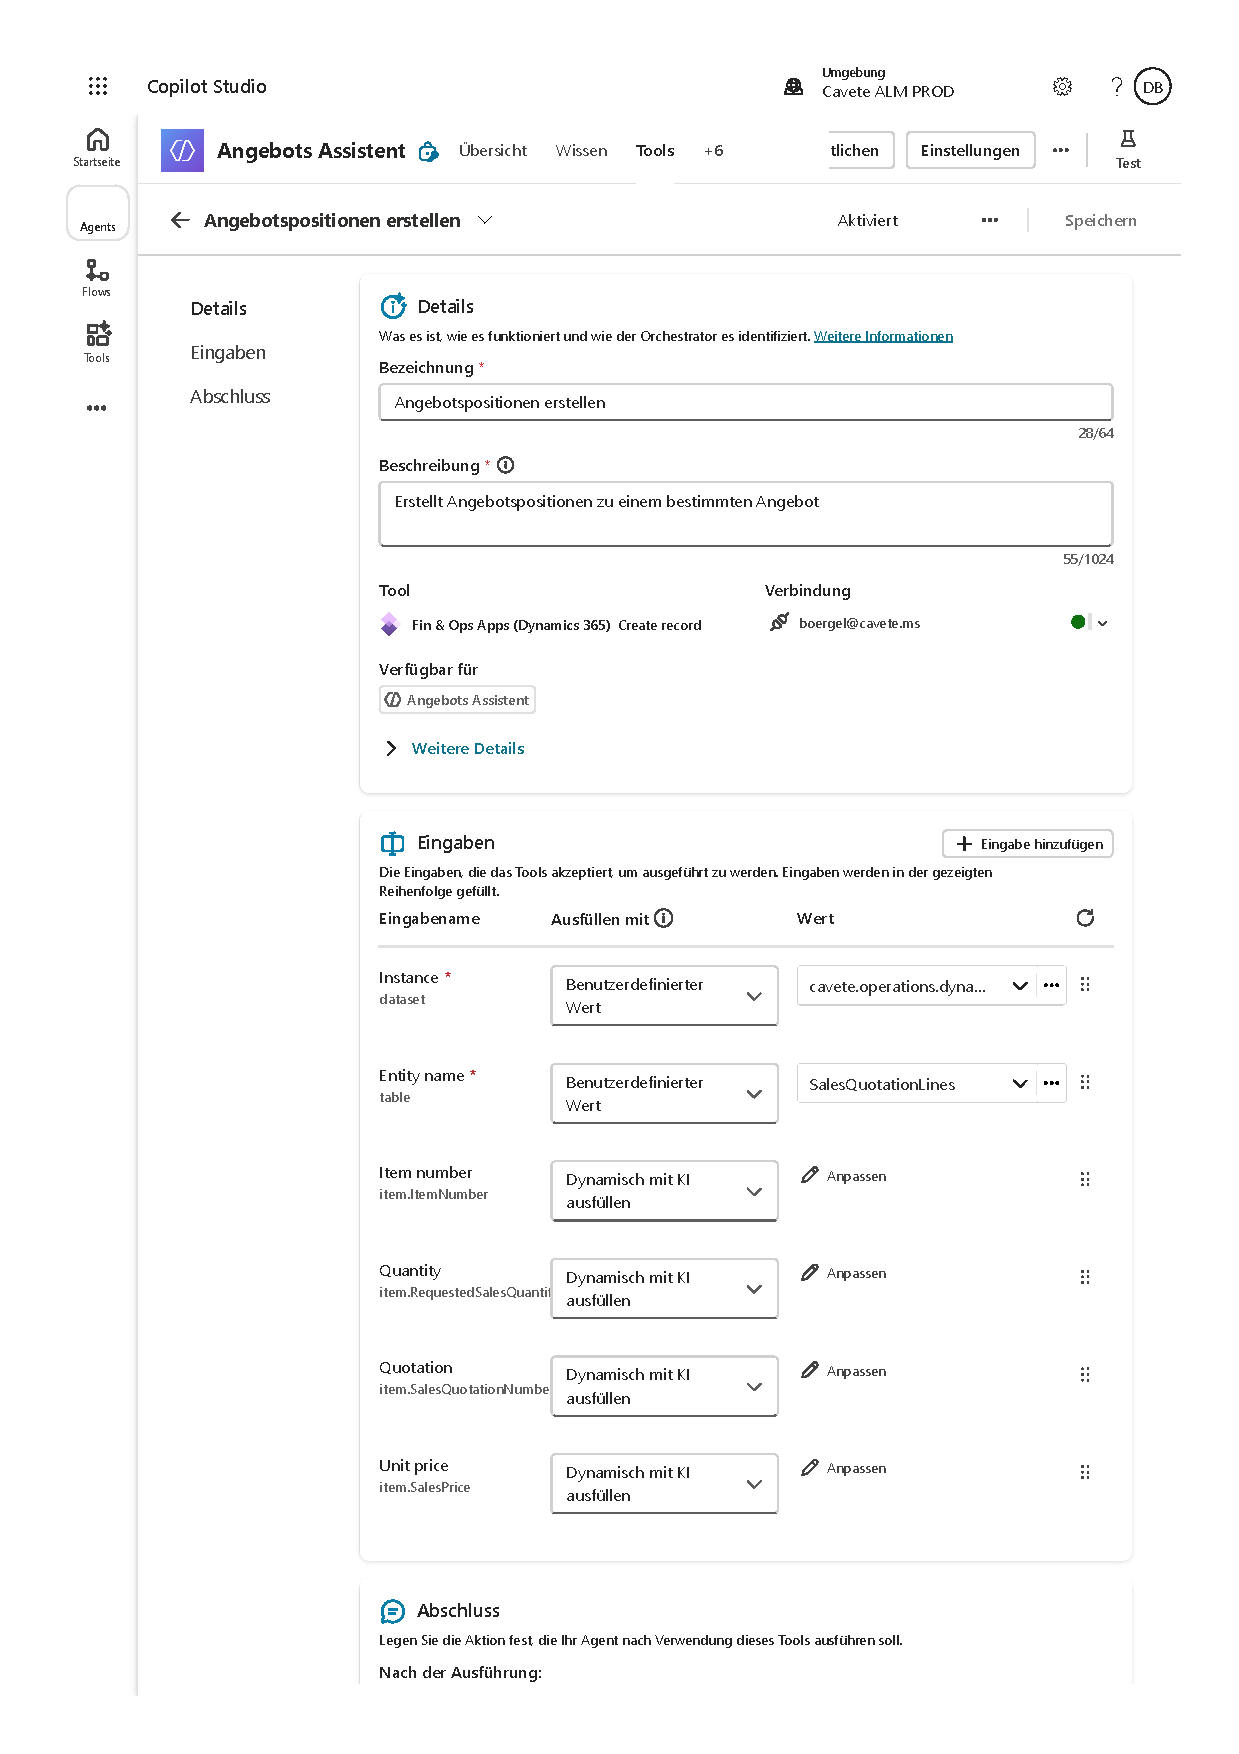
\includegraphics[width=1\textwidth]{kapitel/anhang/images/Angebotspositionen.pdf}
    \caption{Tool: Angebotspositionen erstellen}
    \label{fig:Angebotspositionen}
\end{figure} 

\begin{figure}[H]
    \centering
    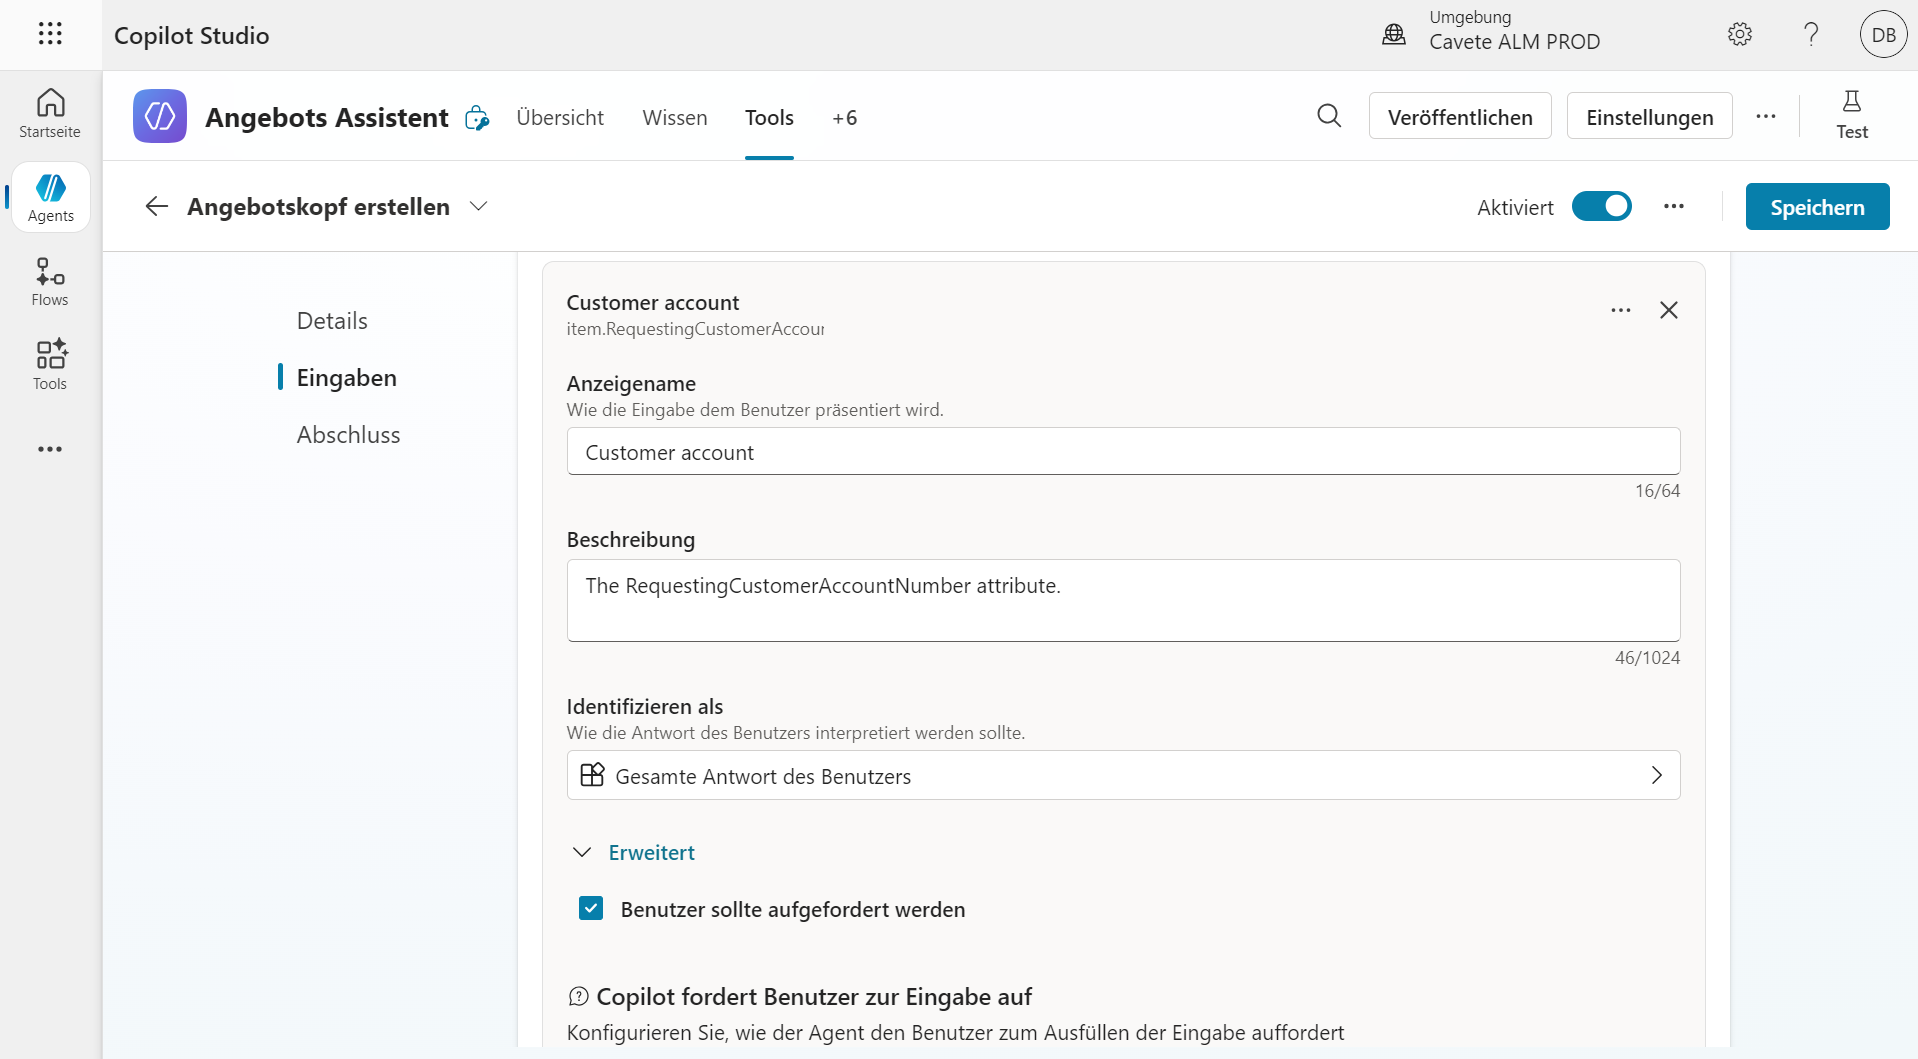
\includegraphics[width=1\textwidth]{kapitel/anhang/images/PflichtfeldTool.png}
    \caption{Tool: Pflichtfelder}
    \label{fig:Pflichtfelder}
\end{figure}

\begin{figure}[H]
    \centering
    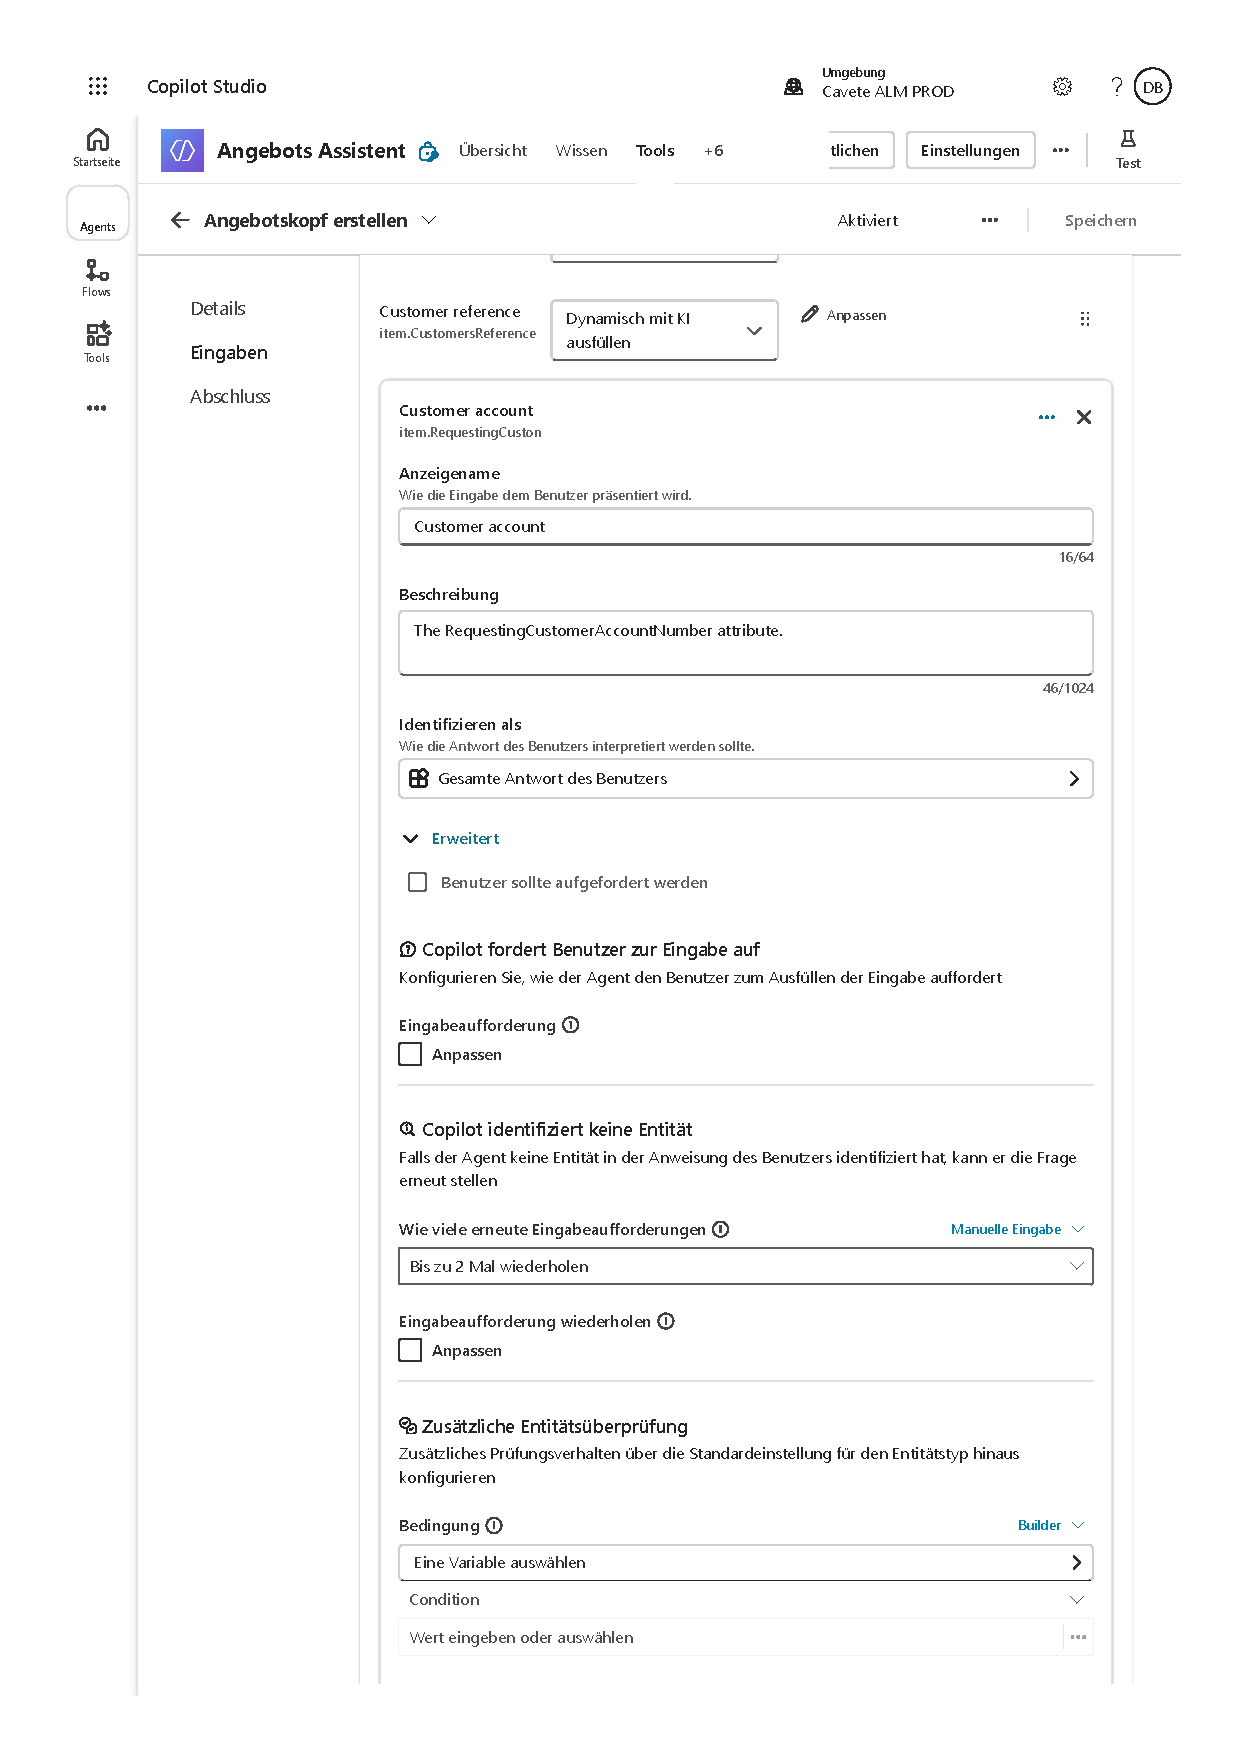
\includegraphics[width=1\textwidth]{kapitel/anhang/images/Zusatzfeld.pdf}
    \caption{Tool: Zusätzliches Feld}
    \label{fig:ZusätzlichesFeld}
\end{figure}  

\begin{figure}[H]
    \centering
    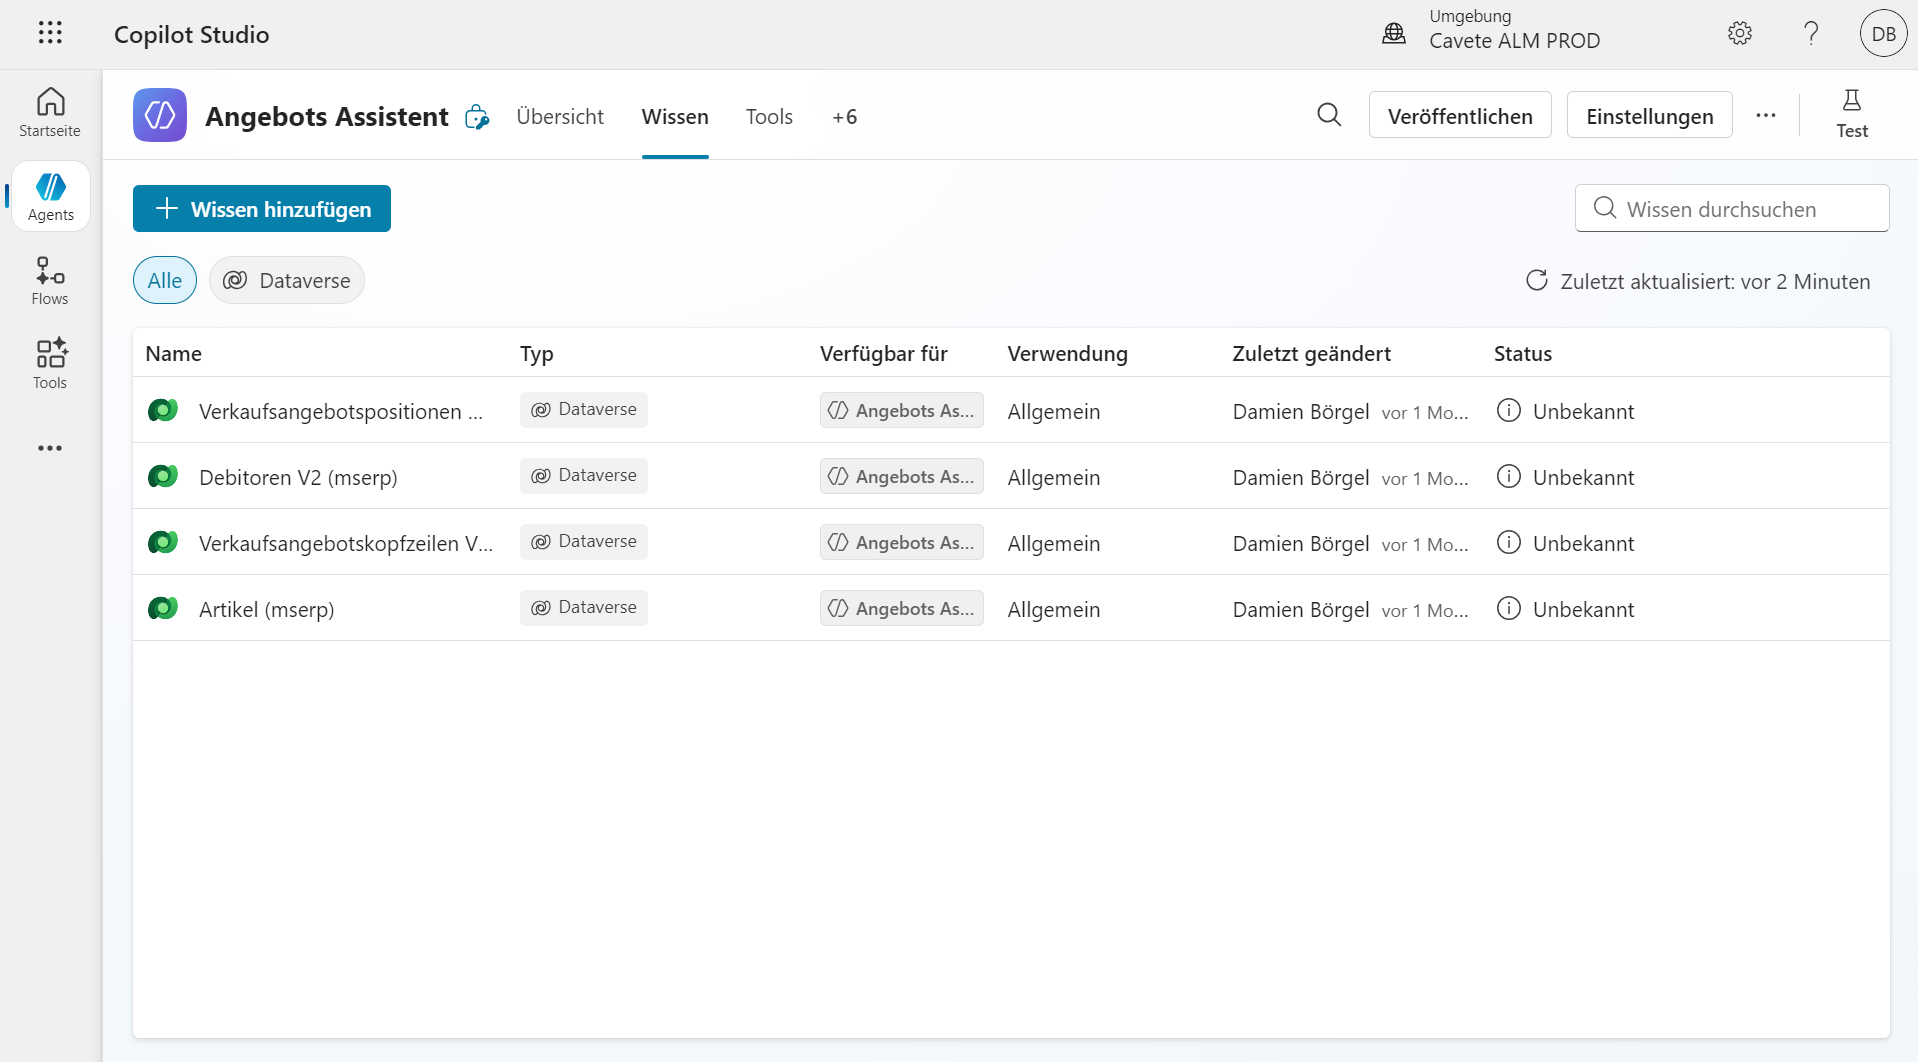
\includegraphics[width=1\textwidth]{kapitel/anhang/images/Wissensquellen.png}
    \caption{Wissensquellen}
    \label{fig:Wissensquellen}
\end{figure}

\begin{figure}[H]
    \centering
    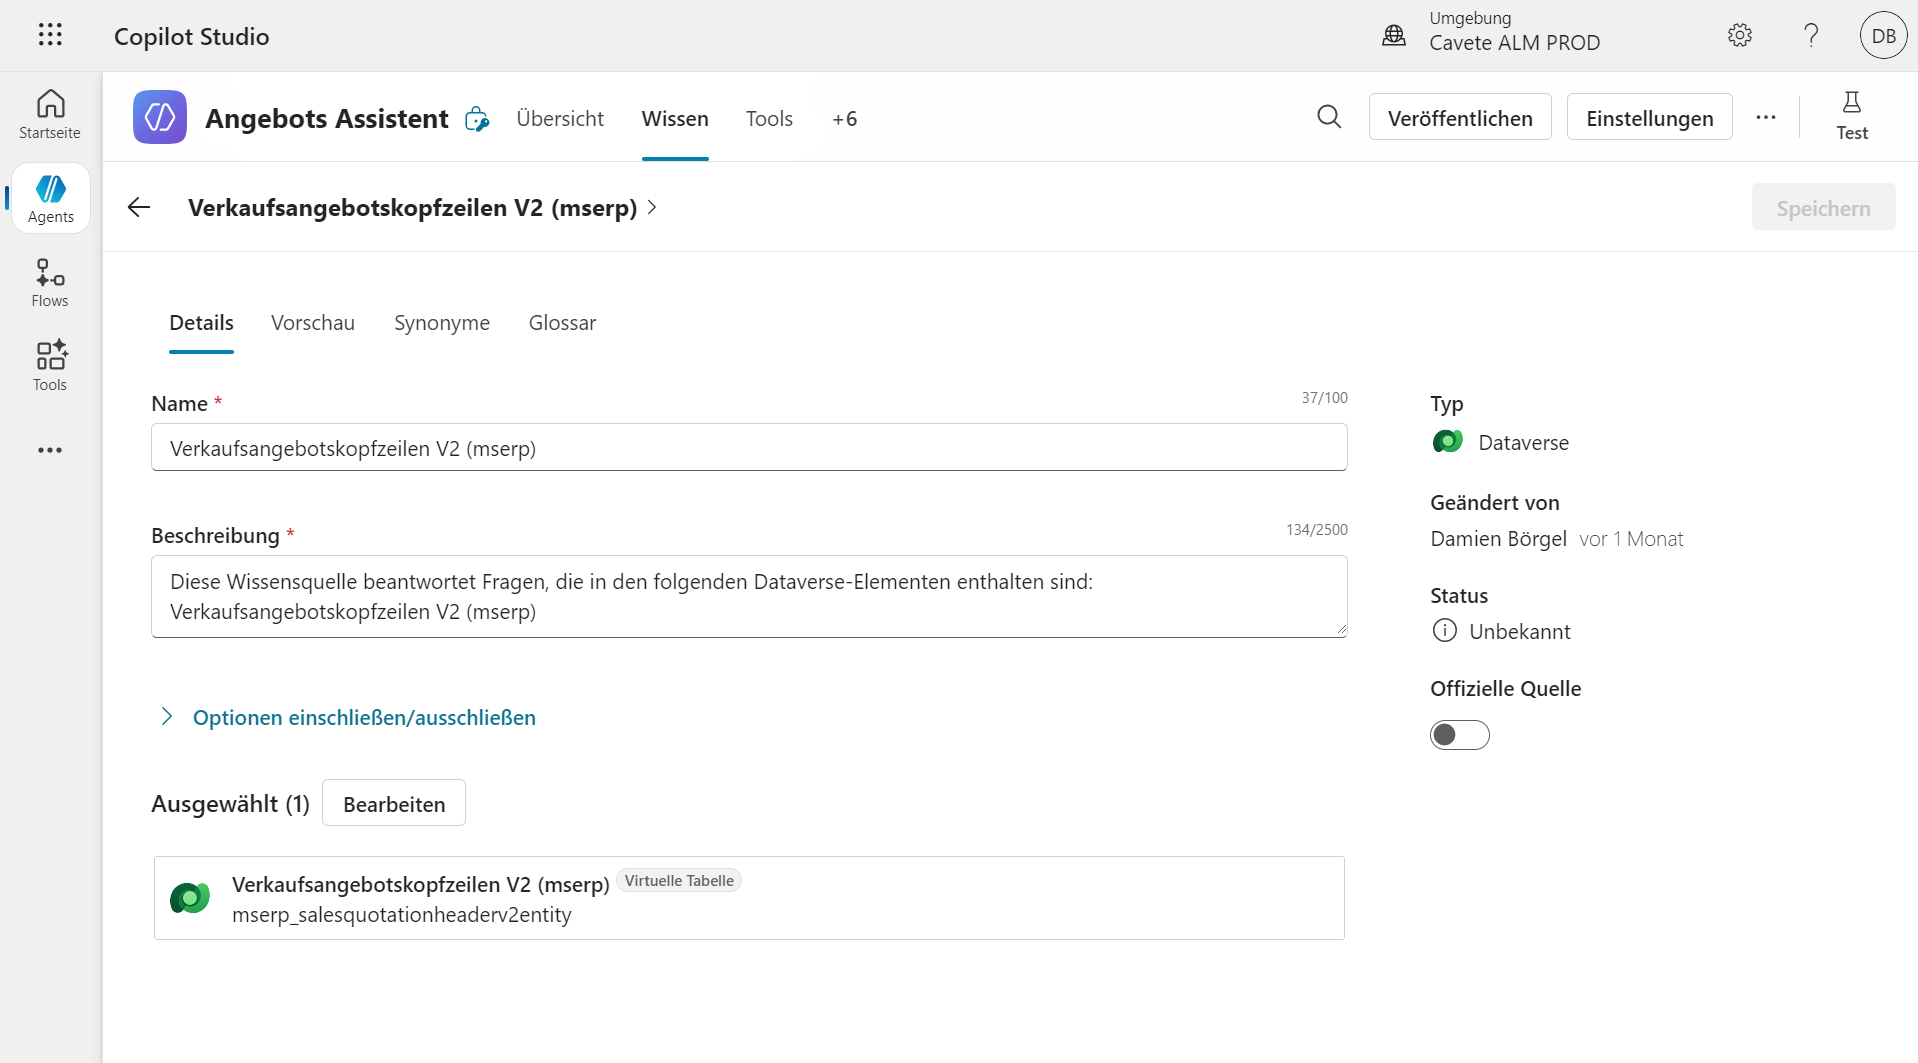
\includegraphics[width=1\textwidth]{kapitel/anhang/images/WissensquelleDetail.png}
    \caption{Wissensquellen: Detailbeispiel}
    \label{fig:WissensquelleDetailbeispiel}
\end{figure}

\begin{figure}[H]
    \centering
    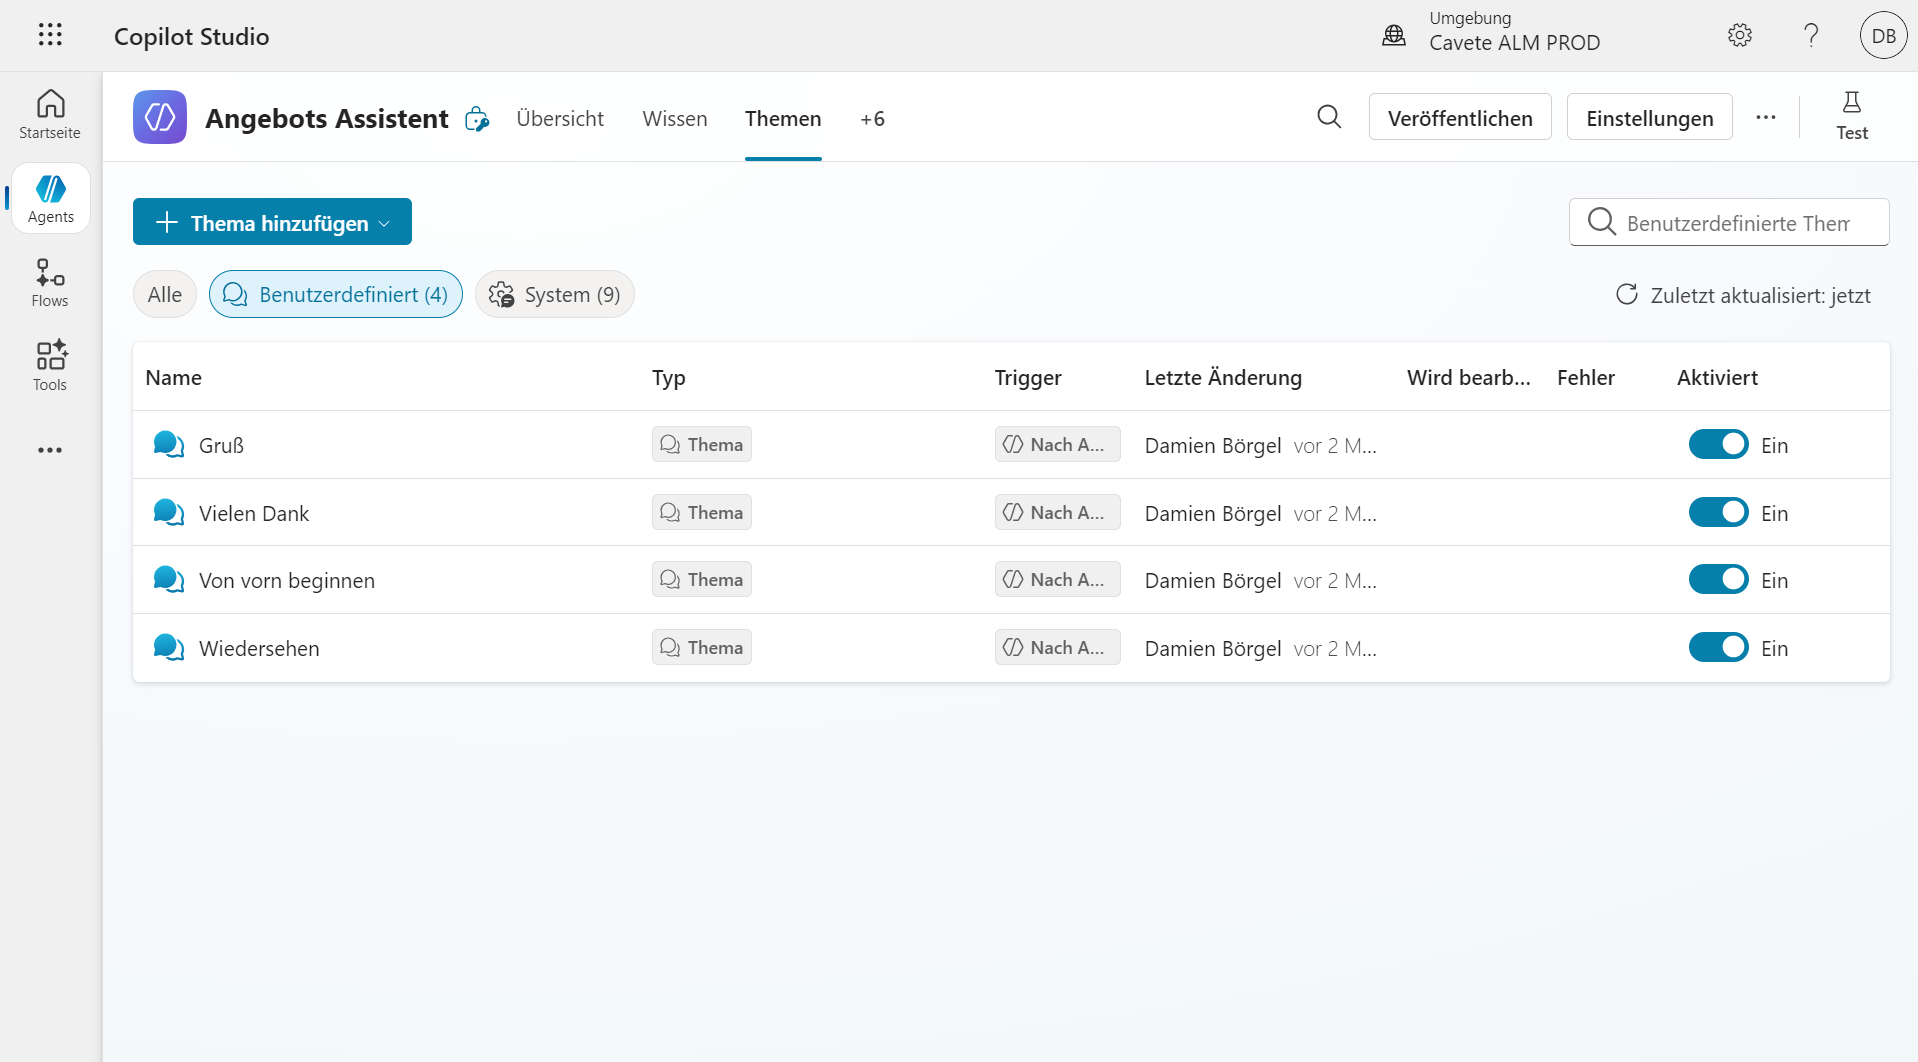
\includegraphics[width=1\textwidth]{kapitel/anhang/images/Topics.png}
    \caption{Topics}
    \label{fig:Topics}
\end{figure}


\begin{figure}[H]
    \centering
    
\includegraphics[width=1\textwidth]{kapitel/anhang/images/CopilotChat1.pdf}
    \caption{Beispielchat1}
    \label{fig:Beispielchat(1/2)}
\end{figure}

\begin{figure}[H]
    \centering
    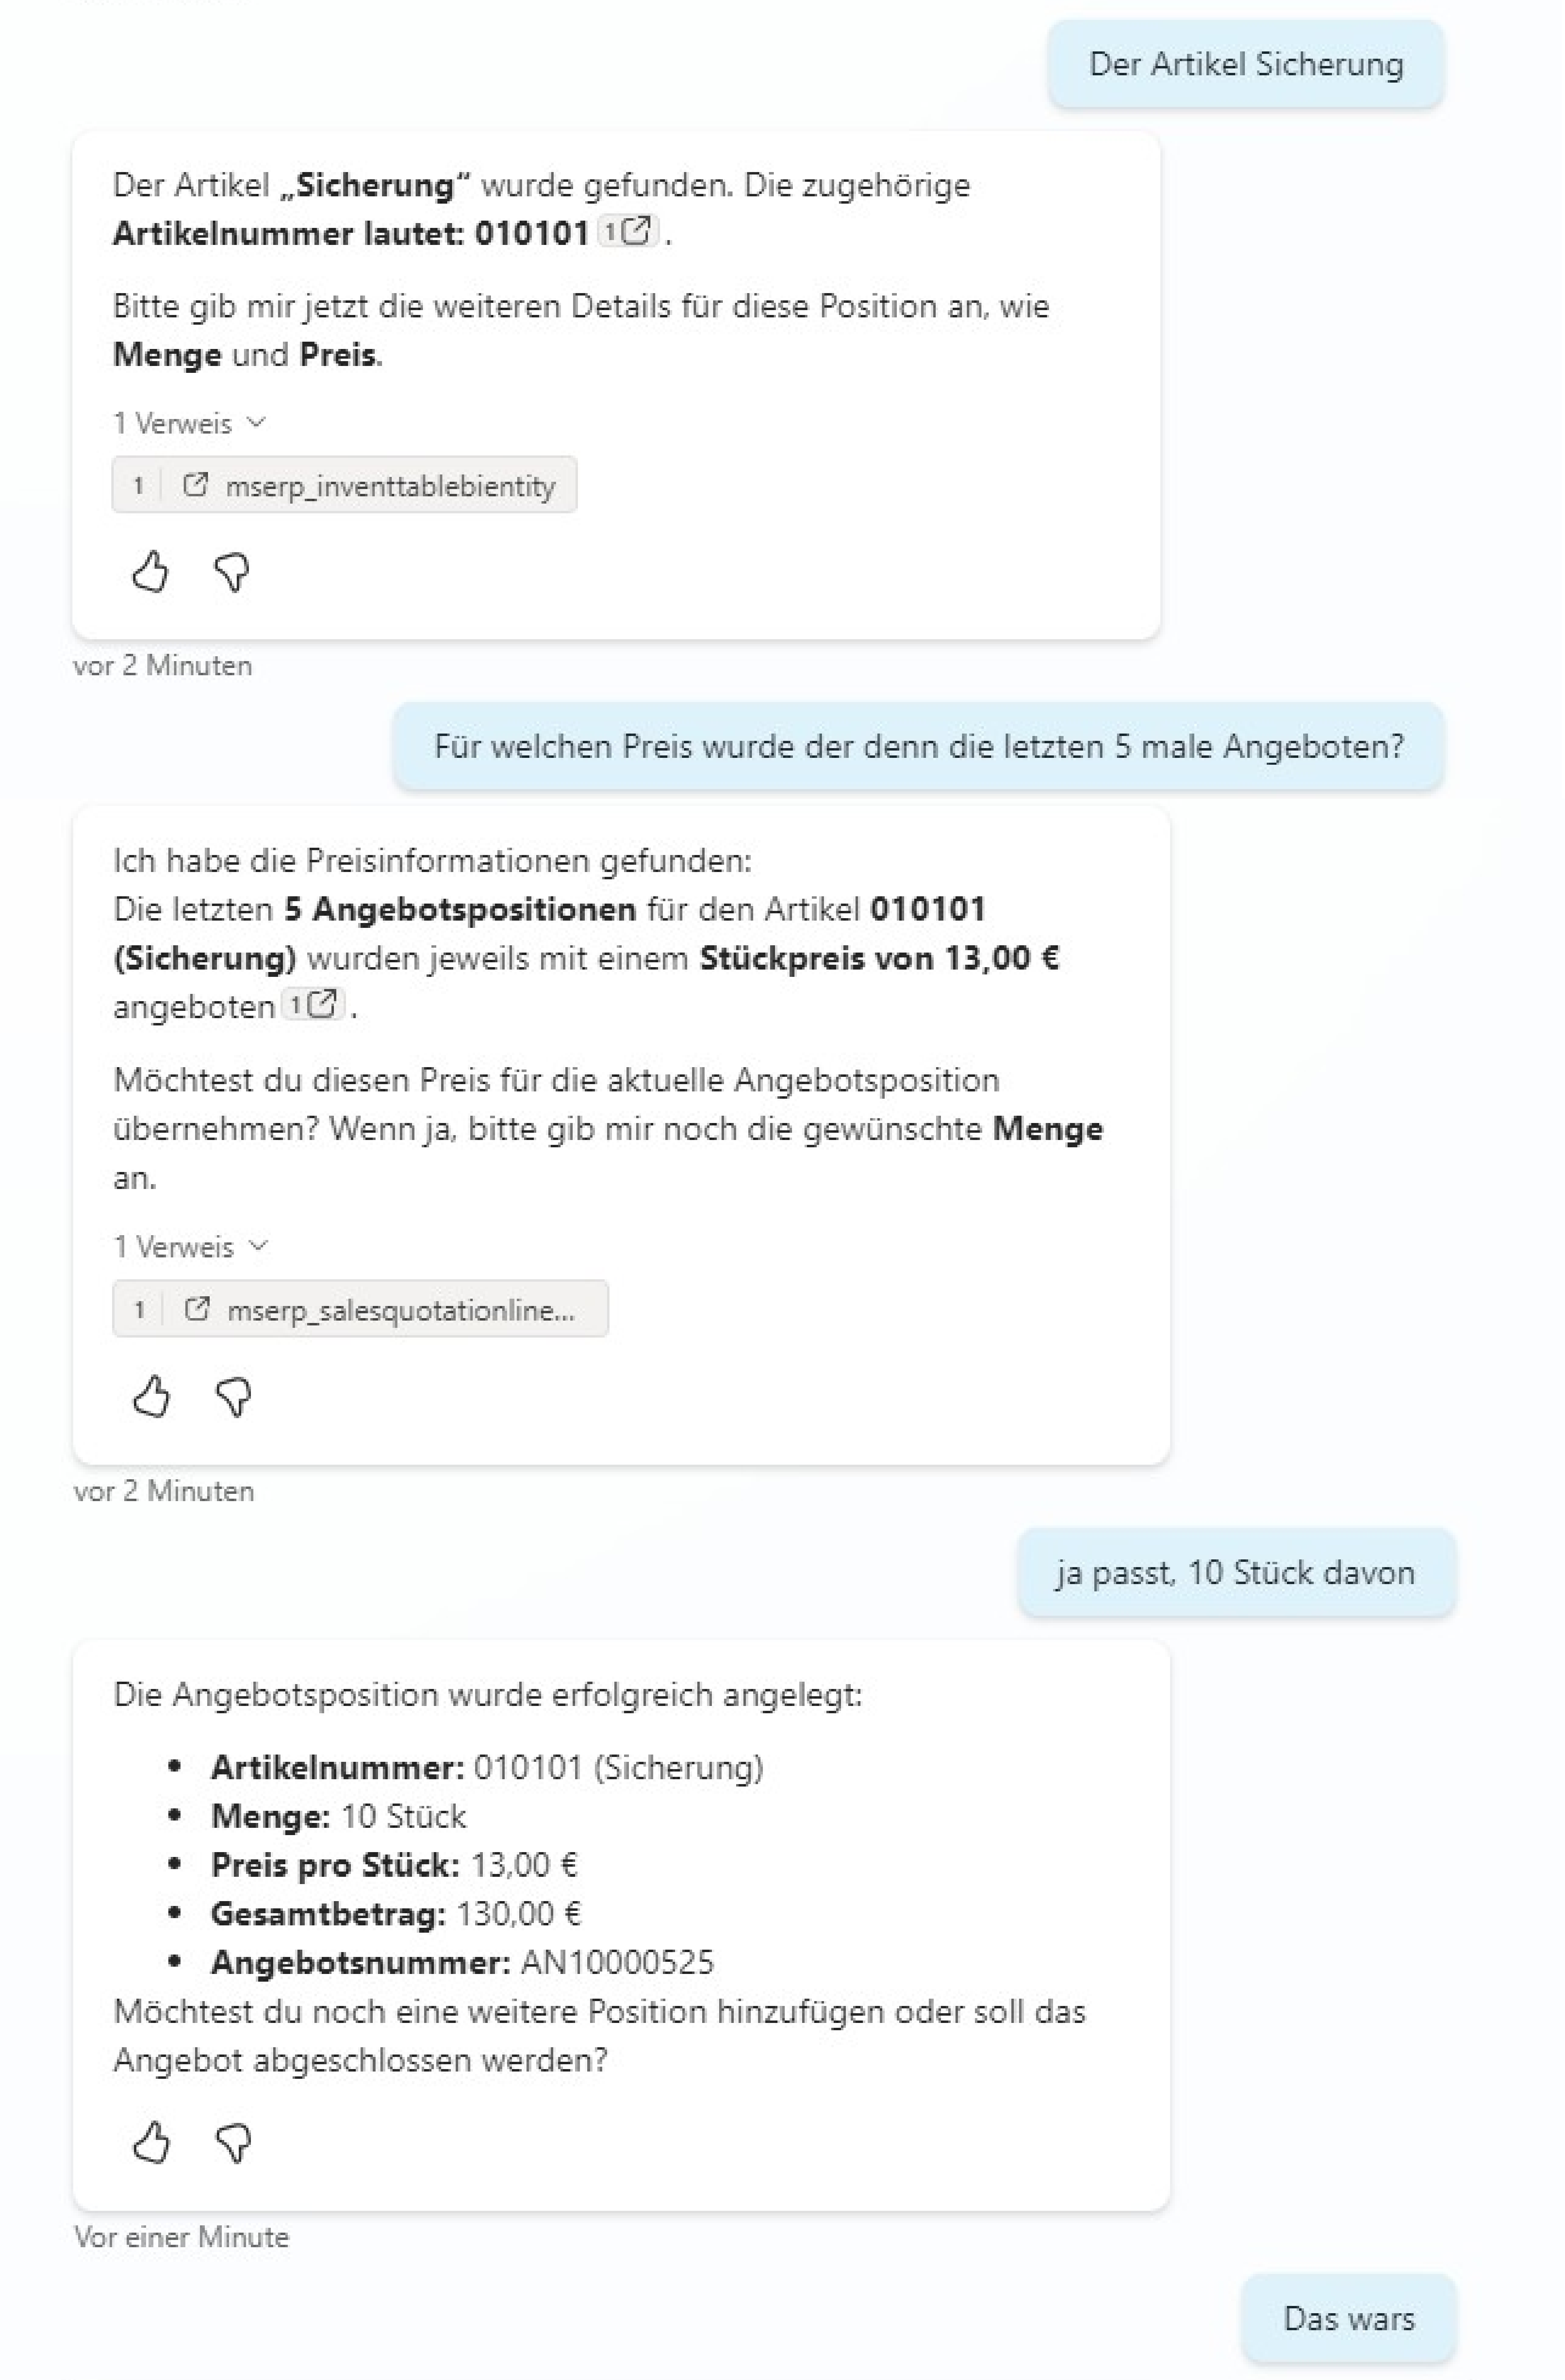
\includegraphics[width=1\textwidth]{kapitel/anhang/images/CopilotChat2.pdf}
    \caption{Beispielchat2}
    \label{fig:Beispielchat (2/2)}
\end{figure}